% PublishJockey System Documentation
% A comprehensive guide to the architecture and functionality
\documentclass[12pt,a4paper]{book}
\usepackage[utf8]{inputenc}
\usepackage[T1]{fontenc}
\usepackage{lmodern}
\usepackage{graphicx}
\usepackage{hyperref}
\usepackage{listings}
\usepackage{color}
\usepackage{xcolor}
\usepackage{tcolorbox}
\usepackage{minted}
\usepackage{amsmath}
\usepackage{amssymb}
\usepackage{booktabs}
\usepackage{tabularx}
\usepackage{tikz}
\usetikzlibrary{shapes,arrows,positioning,fit,backgrounds}

% Define colors for code listings
\definecolor{codebackground}{rgb}{0.95,0.95,0.95}
\definecolor{codekeyword}{rgb}{0.13,0.29,0.53}
\definecolor{codecomment}{rgb}{0.13,0.55,0.13}
\definecolor{codestring}{rgb}{0.63,0.13,0.13}

% Configure code listings
\lstset{
  backgroundcolor=\color{codebackground},
  keywordstyle=\color{codekeyword}\bfseries,
  commentstyle=\color{codecomment},
  stringstyle=\color{codestring},
  basicstyle=\ttfamily\small,
  breaklines=true,
  showstringspaces=false,
  frame=single,
  captionpos=b,
  tabsize=2
}

% Set hyperref options
\hypersetup{
  colorlinks=true,
  linkcolor=blue,
  filecolor=magenta,
  urlcolor=cyan,
  pdftitle={PublishJockey System Documentation},
  pdfauthor={PublishJockey Team}
}

% Document title and author
\title{\Huge \textbf{PublishJockey System Documentation}\\[0.5cm]
\Large A Comprehensive Guide to the Architecture and Functionality}
\author{PublishJockey Development Team}
\date{\today}

\begin{document}

\frontmatter
\maketitle

\tableofcontents

\chapter*{Preface}
\addcontentsline{toc}{chapter}{Preface}

This document serves as the comprehensive technical documentation for the PublishJockey system, a web-based platform designed to help authors create professionally formatted books using markdown editing and LaTeX typesetting technology. It covers the system architecture, components, data models, and key functionality to provide a complete understanding of how PublishJockey works.

The document is intended for developers, system administrators, and technical stakeholders who need to understand, maintain, or extend the PublishJockey platform.

\mainmatter

\chapter{System Overview}

\section{Introduction to PublishJockey}

PublishJockey is a specialized web application designed to simplify the book publishing process. It combines the simplicity of markdown editing with the professional typesetting capabilities of LaTeX to enable authors to create high-quality, print-ready books without requiring technical expertise in typesetting or layout design.

The platform targets authors who need to produce professional-looking books for platforms like Amazon Kindle Direct Publishing (KDP), IngramSpark, and other self-publishing services. PublishJockey handles the complex formatting and typesetting rules automatically, allowing authors to focus on their content.

\section{Key Features}

PublishJockey offers the following key features:

\begin{itemize}
  \item Simple markdown editing interface
  \item Real-time preview of content
  \item Automated LaTeX-powered PDF generation
  \item EPUB and DOCX export options
  \item Support for images, tables, and complex formatting
  \item Customizable book sizes and layouts
  \item KDP-compatible output formats
  \item Subscription-based access model
  \item User account management
  \item ImageMagic tool for upscaling cover images
  \item Document import from Word, Google Docs, and Markdown files
\end{itemize}

\section{System Architecture}

PublishJockey follows a modern microservices architecture, with separate frontend and backend components. The system consists of three main services:

\begin{enumerate}
  \item \textbf{Frontend Application}: A React-based single-page application that provides the user interface
  \item \textbf{Main Backend}: Node.js/Express API server handling authentication, user management, and project storage
  \item \textbf{Export Backend}: Specialized service for document processing, LaTeX compilation, and file export
\end{enumerate}

\begin{figure}[h]
\centering
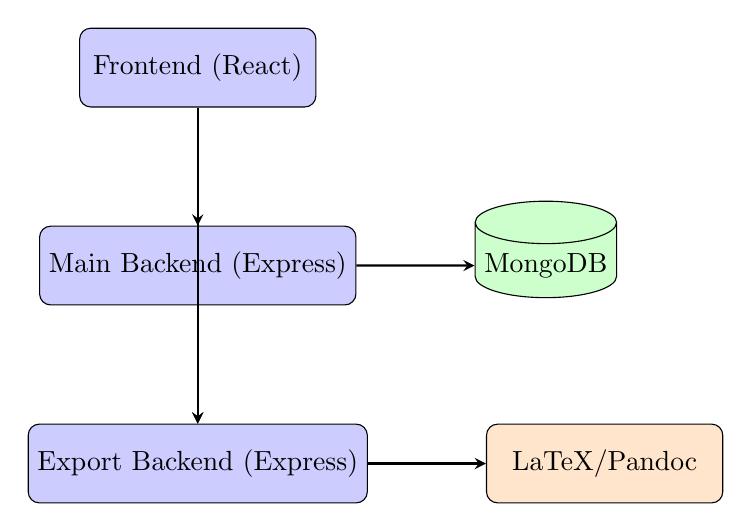
\begin{tikzpicture}[
  node distance=1.5cm,
  service/.style={rectangle, rounded corners, minimum width=3cm, minimum height=1cm, text centered, draw=black, fill=blue!20},
  database/.style={cylinder, shape border rotate=90, aspect=0.3, minimum height=1cm, minimum width=1.5cm, draw=black, fill=green!20},
  arrow/.style={thick,->,>=stealth}
]
% Services
\node (frontend) [service] {Frontend (React)};
\node (backend) [service, below=of frontend] {Main Backend (Express)};
\node (export) [service, below=of backend] {Export Backend (Express)};

% Databases
\node (mongodb) [database, right=of backend] {MongoDB};

% External Services
\node (latex) [service, right=of export, fill=orange!20] {LaTeX/Pandoc};

% Connections
\draw [arrow] (frontend) -- (backend);
\draw [arrow] (frontend) -- (export);
\draw [arrow] (backend) -- (mongodb);
\draw [arrow] (backend) -- (export);
\draw [arrow] (export) -- (latex);

\end{tikzpicture}
\caption{PublishJockey System Architecture}
\end{figure}

\section{Technology Stack}

PublishJockey is built on a modern web technology stack:

\begin{itemize}
  \item \textbf{Frontend}: React, Material-UI, JavaScript/TypeScript
  \item \textbf{Backend}: Node.js, Express.js, MongoDB
  \item \textbf{Export Processing}: LaTeX, Pandoc, Node.js
  \item \textbf{Authentication}: JWT (JSON Web Tokens)
  \item \textbf{Deployment}: Docker, Nginx
  \item \textbf{Version Control}: Git
\end{itemize}

\chapter{Data Models}

\section{Core Data Models}

PublishJockey's data architecture is centered around several key models that represent the core entities in the system.

\subsection{User Model}

The User model represents registered users of the system and contains authentication and subscription information.

\begin{lstlisting}[language=JavaScript, caption=User Schema]
const UserSchema = new mongoose.Schema({
  name: {
    type: String,
    required: [true, 'Please provide a name'],
    trim: true,
    maxlength: [50, 'Name cannot be more than 50 characters']
  },
  email: {
    type: String,
    required: [true, 'Please provide an email'],
    match: [
      /^(([^<>()[\]\\.,;:\s@"]+(\.[^<>()[\]\\.,;:\s@"]+)*)|(".+"))@((\[[0-9]{1,3}\.[0-9]{1,3}\.[0-9]{1,3}\.[0-9]{1,3}\])|(([a-zA-Z\-0-9]+\.)+[a-zA-Z]{2,}))$/,
      'Please provide a valid email'
    ],
    unique: true,
    lowercase: true,
    trim: true
  },
  password: {
    type: String,
    required: [true, 'Please provide a password'],
    minlength: [8, 'Password must be at least 8 characters'],
    select: false
  },
  role: {
    type: String,
    enum: ['user', 'admin'],
    default: 'user'
  },
  subscription: {
    type: String,
    enum: ['free', 'beta', 'author', 'starter', 'growth', 'professional', 'power', 'custom'],
    default: 'free'
  },
  booksRemaining: {
    type: Number,
    default: 1, // Default for free plan is 1 book
  },
  booksAllowed: {
    type: Number,
    default: 1, // Default for free plan is 1 book
  },
  subscriptionExpires: {
    type: Date,
    default: () => {
      const date = new Date();
      date.setFullYear(date.getFullYear() + 100); // Free subscription "expires" in 100 years
      return date;
    }
  },
  // Additional fields for account management and security
  isVerified: Boolean,
  verificationToken: String,
  verificationTokenExpires: Date,
  resetPasswordToken: String,
  resetPasswordExpires: Date,
  createdAt: Date,
  isSuspended: Boolean,
  suspensionReason: String,
  lastLogin: Date,
  loginAttempts: Number,
  accountLocked: Boolean,
  accountLockedUntil: Date,
  notifications: [
    {
      title: String,
      message: String,
      read: Boolean,
      createdAt: Date
    }
  ]
});
\end{lstlisting}

\subsection{Project Model}

The Project model represents a book project, containing metadata and content structure.

\begin{lstlisting}[language=JavaScript, caption=Project Schema]
const ProjectSchema = new Schema({
  title: {
    type: String,
    required: [true, 'Project title is required'],
    trim: true,
    maxlength: [100, 'Project title cannot be more than 100 characters']
  },
  author: {
    type: String,
    default: ''
  },
  subtitle: {
    type: String,
    default: ''
  },
  isbn: {
    type: String,
    default: ''
  },
  description: {
    type: String,
    required: false,
    default: '',
    trim: true
  },
  status: {
    type: String,
    enum: ['planning', 'in-progress', 'completed', 'on-hold'],
    default: 'planning'
  },
  owner: {
    type: Schema.Types.ObjectId,
    ref: 'User',
    required: false,
    default: null
  },
  userId: {
    type: Schema.Types.ObjectId,
    ref: 'User',
    required: false
  },
  collaborators: [{
    type: Schema.Types.ObjectId,
    ref: 'User'
  }],
  createdAt: {
    type: Date,
    default: Date.now
  },
  updatedAt: {
    type: Date,
    default: Date.now
  },
  content: {
    type: Object,
    default: {}
  },
  structure: {
    type: Object,
    default: {
      front: ["Title Page", "Copyright", "Dedication", "Acknowledgments"],
      main: ["Chapter 1", "Chapter 2", "Chapter 3"],
      back: ["About the Author"]
    }
  }
}, {
  timestamps: true
});
\end{lstlisting}

\section{Subscription and Pricing Model}

PublishJockey implements a tiered subscription model with the following plans:

\begin{table}[h]
\centering
\begin{tabularx}{\textwidth}{|X|X|X|X|}
\hline
\textbf{Plan} & \textbf{Price} & \textbf{Books Allowed} & \textbf{Features} \\
\hline
Free & \$0 & 1 (limited to first 10 pages) & Basic features, watermarked exports \\
\hline
Author & \$79 (one-time) & 1 & Full book export, watermark-free output \\
\hline
Starter & \$299 & 5 & Multiple books, standard support \\
\hline
Growth & \$499 & 10 & Priority support, enhanced storage \\
\hline
Professional & \$699 & 20 & Premium support, bulk formatting tools \\
\hline
Power Publisher & \$899 & 30 & VIP support, advanced customization \\
\hline
Custom & Custom & 30+ & Dedicated account manager, custom integrations \\
\hline
\end{tabularx}
\caption{PublishJockey Subscription Plans}
\end{table}

\chapter{Frontend Application}

\section{User Interface Components}

The PublishJockey frontend is built using React and Material-UI, providing a responsive and modern user interface. The main components include:

\begin{itemize}
  \item Landing page with features, pricing, and testimonials
  \item User authentication (login/registration)
  \item Dashboard for project management
  \item Markdown editor with real-time preview
  \item Export configuration interface
  \item User account and subscription management
\end{itemize}

\section{Landing Page}

The landing page serves as the main entry point for new users, showcasing the platform's features, pricing, and testimonials. It includes the following sections:

\begin{itemize}
  \item Hero section with call-to-action
  \item Features overview
  \item How it works step-by-step guide
  \item Pricing plans
  \item Testimonials from users
  \item Frequently asked questions
\end{itemize}

The landing page is designed to convert visitors into registered users by highlighting the value proposition and addressing common questions.

\section{Markdown Editor}

The markdown editor is the core component of the application, providing a simple yet powerful interface for authors to write and format their content. Key features include:

\begin{itemize}
  \item Split-pane view with editor and preview
  \item Syntax highlighting for markdown
  \item Toolbar for common formatting options
  \item Image upload and management
  \item Table creation and editing
  \item Section navigation and management
\end{itemize}

\section{Project Management}

The project management interface allows users to:

\begin{itemize}
  \item Create new book projects
  \item Organize content into front matter, main content, and back matter
  \item Add, remove, and reorder sections
  \item Set book metadata (title, author, ISBN, etc.)
  \item Configure export settings
\end{itemize}

\chapter{Backend Services}

\section{Main Backend}

The main backend service handles user authentication, project management, and data storage. It provides RESTful APIs for the frontend to interact with.

\subsection{Authentication System}

PublishJockey implements a secure JWT-based authentication system with the following features:

\begin{itemize}
  \item User registration with email verification
  \item Login with rate limiting to prevent brute force attacks
  \item Password reset functionality
  \item Token-based authentication with refresh tokens
  \item Role-based access control (user/admin)
\end{itemize}

\subsection{Project Management}

The project management APIs allow users to:

\begin{itemize}
  \item Create, read, update, and delete book projects
  \item Manage project metadata
  \item Save and retrieve content for each section
  \item Organize the structure of their book
\end{itemize}

\subsection{User Management}

Admin users have access to user management features:

\begin{itemize}
  \item View and search user accounts
  \item Manage user subscriptions
  \item Reset user passwords
  \item Suspend or delete accounts
\end{itemize}

\section{Export Backend}

The export backend is a specialized service focused on document processing and export. It handles the complex task of converting markdown content to various output formats.

\subsection{Document Import}

The import functionality supports multiple input formats:

\begin{itemize}
  \item Microsoft Word (.docx) using Pandoc
  \item Google Docs via URL
  \item Markdown files
  \item Plain text files
\end{itemize}

\subsection{PDF Export}

The PDF export process is the most sophisticated part of the system, leveraging LaTeX for professional typesetting:

\begin{enumerate}
  \item Assemble markdown content from all sections
  \item Process markdown to enhance formatting
  \item Generate LaTeX code with appropriate settings
  \item Compile LaTeX to PDF using Pandoc
  \item Apply appropriate page size, margins, and formatting
\end{enumerate}

\begin{lstlisting}[language=JavaScript, caption=PDF Export Function]
function exportPdf(assembledPath, outputPath, options = {}) {
  return new Promise(async (resolve, reject) => {
    try {
      // Default options
      const {
        pageSize = "6x9",
        includeToc = true,
        tocDepth = 3,
        fontFamily = "default",
        fontSize = "11pt",
        lineSpacing = "1.15",
        chapterLabelFormat = "number", // "number", "text", or "none"
        hasPageNumbers = true,
        customMargins = null,
        debugMode = false
      } = options;

      // Estimate page count for margin calculation
      const content = fs.readFileSync(assembledPath, 'utf8');
      const estimatedPages = estimatePageCount(content, pageSize, includeToc);
      
      // Generate pandoc command arguments
      const pandocArgs = [
        '--pdf-engine=xelatex',
        '-f', 'markdown',
        '-t', 'pdf',
        '-o', outputPath,
        '--toc-depth=' + tocDepth,
        '--variable=documentclass:book',
        '--variable=papersize:' + pageSize,
        '--variable=fontsize:' + fontSize,
        '--variable=linestretch:' + lineSpacing,
        // Additional variables for page geometry, fonts, etc.
      ];
      
      // Execute pandoc command
      execFile('pandoc', pandocArgs, { maxBuffer: 10 * 1024 * 1024 }, (error, stdout, stderr) => {
        if (error) {
          console.error('PDF export error:', error);
          reject(error);
        } else {
          resolve(outputPath);
        }
      });
    } catch (error) {
      reject(error);
    }
  });
}
\end{lstlisting}

\subsection{EPUB Export}

The EPUB export process creates e-book compatible files:

\begin{enumerate}
  \item Assemble markdown content
  \item Convert to HTML using marked library
  \item Generate EPUB using epub-gen library
  \item Apply appropriate styling and metadata
\end{enumerate}

\subsection{DOCX Export}

The DOCX export provides Microsoft Word compatibility:

\begin{enumerate}
  \item Assemble markdown content
  \item Use Pandoc to convert markdown to DOCX
  \item Apply basic styling and formatting
\end{enumerate}

\chapter{Key Functionality}

\section{Book Assembly Process}

The book assembly process is a core functionality that combines multiple markdown sections into a cohesive document:

\begin{enumerate}
  \item Retrieve all sections for a project
  \item Organize sections based on the book structure (front matter, main content, back matter)
  \item Process each section's markdown content
  \item Combine sections with appropriate formatting and page breaks
  \item Add table of contents if requested
\end{enumerate}

\section{Markdown Processing}

PublishJockey enhances standard markdown with special processing for book formatting:

\begin{itemize}
  \item Chapter numbering and formatting
  \item Image handling with captions
  \item Table formatting
  \item Block quotes and callouts
  \item Centered and right-aligned text
\end{itemize}

\section{LaTeX Integration}

The system uses LaTeX for professional typesetting, with custom templates and configurations:

\begin{itemize}
  \item Book template with proper front matter, main content, and back matter
  \item Dynamic margin calculation based on page count and book size
  \item Custom LaTeX commands for special formatting
  \item Font selection and configuration
\end{itemize}

\section{ImageMagic Tool}

The ImageMagic tool is a specialized feature for upscaling low-resolution cover images:

\begin{itemize}
  \item Accepts PNG and JPG input
  \item Automatically detects book dimensions
  \item Upscales images to 300 DPI for print quality
  \item Preserves image quality using advanced algorithms
\end{itemize}

\section{Fair Use Protection}

PublishJockey implements a fair use protection system to enforce subscription limits:

\begin{itemize}
  \item AI-powered monitoring of book content
  \item Tracking of book exports per user
  \item Enforcement of book limits based on subscription
  \item Prevention of subscription abuse
\end{itemize}

\chapter{Deployment and Infrastructure}

\section{Development Environment}

The development environment setup includes:

\begin{itemize}
  \item Node.js and npm for JavaScript development
  \item MongoDB for database
  \item LaTeX/Pandoc installation for export functionality
  \item Git for version control
\end{itemize}

\section{Production Deployment}

The production deployment architecture consists of:

\begin{itemize}
  \item Frontend hosted on a static file server or CDN
  \item Backend services deployed as Docker containers
  \item MongoDB database (could be self-hosted or cloud service)
  \item Nginx as reverse proxy and static file server
  \item SSL/TLS encryption for secure connections
\end{itemize}

\section{Scaling Considerations}

For scaling the system to handle more users:

\begin{itemize}
  \item Horizontal scaling of backend services
  \item Database sharding for large data volumes
  \item Caching layer for frequently accessed data
  \item Queue system for export jobs to prevent overload
  \item CDN for static assets and exported files
\end{itemize}

\chapter{Security Considerations}

\section{Authentication and Authorization}

PublishJockey implements several security measures for authentication:

\begin{itemize}
  \item Password hashing using bcrypt
  \item JWT tokens with appropriate expiration
  \item CSRF protection
  \item Rate limiting for login attempts
  \item Role-based access control
\end{itemize}

\section{Data Protection}

Data protection measures include:

\begin{itemize}
  \item HTTPS for all communications
  \item Sanitization of user inputs
  \item Validation of file uploads
  \item Secure handling of user content
  \item Regular security audits
\end{itemize}

\chapter{Future Development}

\section{Planned Enhancements}

Future development plans for PublishJockey include:

\begin{itemize}
  \item Enhanced collaboration features
  \item Integration with additional publishing platforms
  \item Advanced typesetting options for academic publications
  \item AI-assisted writing and editing tools
  \item Mobile application for on-the-go editing
\end{itemize}

\section{Technical Roadmap}

The technical roadmap includes:

\begin{itemize}
  \item Migration to TypeScript for improved type safety
  \item Implementation of GraphQL API for more efficient data fetching
  \item Enhanced testing coverage
  \item Performance optimizations for large documents
  \item Improved error handling and user feedback
\end{itemize}

\appendix

\chapter{API Reference}

\section{Authentication API}

\begin{table}[h]
\centering
\begin{tabularx}{\textwidth}{|l|X|X|}
\hline
\textbf{Endpoint} & \textbf{Method} & \textbf{Description} \\
\hline
/api/auth/register & POST & Register a new user \\
\hline
/api/auth/login & POST & Authenticate user and get tokens \\
\hline
/api/auth/refresh & POST & Refresh access token \\
\hline
/api/auth/verify & GET & Verify email address \\
\hline
/api/auth/forgot-password & POST & Request password reset \\
\hline
/api/auth/reset-password & POST & Reset password with token \\
\hline
\end{tabularx}
\caption{Authentication API Endpoints}
\end{table}

\section{Project API}

\begin{table}[h]
\centering
\begin{tabularx}{\textwidth}{|l|X|X|}
\hline
\textbf{Endpoint} & \textbf{Method} & \textbf{Description} \\
\hline
/api/projects & GET & List user's projects \\
\hline
/api/projects & POST & Create a new project \\
\hline
/api/projects/:id & GET & Get project details \\
\hline
/api/projects/:id & PUT & Update project \\
\hline
/api/projects/:id & DELETE & Delete project \\
\hline
/api/projects/:id/content & GET & Get project content \\
\hline
/api/projects/:id/content & PUT & Update project content \\
\hline
/api/projects/:id/export & POST & Export project \\
\hline
\end{tabularx}
\caption{Project API Endpoints}
\end{table}

\chapter{Troubleshooting Guide}

\section{Common Issues}

\begin{itemize}
  \item PDF export fails: Check LaTeX installation and temporary file permissions
  \item Image upload issues: Verify file size limits and supported formats
  \item Authentication problems: Check token expiration and server logs
  \item MongoDB connection errors: Verify database connection string and credentials
\end{itemize}

\section{Debugging Tools}

\begin{itemize}
  \item Server logs for backend issues
  \item Browser developer tools for frontend debugging
  \item MongoDB Compass for database inspection
  \item Postman for API testing
\end{itemize}

\backmatter

\chapter*{Glossary}
\addcontentsline{toc}{chapter}{Glossary}

\begin{description}
  \item[KDP] Kindle Direct Publishing, Amazon's self-publishing platform
  \item[LaTeX] A document preparation system for high-quality typesetting
  \item[Markdown] A lightweight markup language for creating formatted text
  \item[Pandoc] A universal document converter used for format conversion
  \item[JWT] JSON Web Token, used for secure authentication
  \item[EPUB] Electronic publication, a digital book format
  \item[DOCX] Microsoft Word document format
  \item[DPI] Dots Per Inch, a measure of image resolution
\end{description}

\chapter*{Index}
\addcontentsline{toc}{chapter}{Index}

\end{document}